% arXiv v1 source (2026-11-16).
% Every number traces to experiments/validate_theorem1.py (final mode),
% validate_drift_deficiency.py, validate_tv_gap.py (results/tv_gap.csv),
% wilds_benchmark.py (exact LP, 5 bins, 20 bootstrap, seed 42) and
% make_benchmark_figures.py, as run by reproduce.sh; proofs/check_manuscript_numbers.py
% prints every quoted value from the result files.
\documentclass{article}
\usepackage[margin=1in]{geometry}
\usepackage{amsmath, amsthm, amssymb}
\usepackage{hyperref}
\usepackage{graphicx}
\usepackage{booktabs}
\usepackage[numbers,sort&compress]{natbib}

\newtheorem{theorem}{Theorem}
\newtheorem{proposition}[theorem]{Proposition}
\newtheorem{corollary}[theorem]{Corollary}
\newtheorem{definition}{Definition}
\newtheorem{remark}{Remark}

\renewcommand{\P}{\mathbb{P}}
\newcommand{\TV}[2]{\|#1 - #2\|_{\mathrm{TV}}}
\newcommand{\Pcal}{P_{\mathrm{cal}}}
\newcommand{\Ptest}{P_{\mathrm{test}}}

\title{Coverage Validity Under Distribution Shift:\\
Deficiency as a Shift-Severity Monitor for Conformal Predictors}

\author{
  Deniz Akdemir\\
  Independent Researcher\\
  \texttt{deniz.akdemir.work@gmail.com}
}
\date{}

\begin{document}
\maketitle

\begin{abstract}
Split conformal prediction guarantees coverage only under exchangeability, and
deployment shift can erode it silently. We record three things. First, coverage
loss is bounded by the joint total variation (TV) between calibration and test
distributions with coefficient one, and that coefficient cannot be improved.
Second, the experiment deficiency of Le Cam theory, estimated from
class-conditional histograms, does \emph{not} bound that TV: it is never larger
than the largest class-conditional TV, and it is exactly zero when classes have
disjoint support, however large the shift. In a controlled Gaussian example
the estimate is 4--8\% of the true joint TV, so a ``$2\hat\delta$'' bound is
violated in essentially every trial at moderate shift. Third, despite this, the
estimate is a useful but uncertified monitor in some settings: it rises with
shift in the synthetic experiments and ranks domain difficulty on one real
tabular benchmark, while on a text benchmark it does not track coverage loss
at all. The estimator and the conformal, calibration and drift tools are
implemented in an open-source Python package, ReliabilityLayer, and we
report where the monitor fails.
\end{abstract}

\section{Introduction}

Conformal prediction adds distribution-free uncertainty sets to arbitrary
predictive models \citep{vovk2005algorithmic,angelopoulos2021gentle}. In
deployment, calibration and test data are not exchangeable, and empirical
coverage can fall below the nominal level. Weighted conformal methods correct
for covariate shift given a density ratio \citep{tibshirani2019conformal},
online methods adapt with feedback \citep{gibbs2021adaptive}, and
TV-based analyses give worst-case coverage bounds
\citep{barber2023conformal}. What a practitioner lacks is a model-agnostic
quantity that can be \emph{monitored} to indicate how far the calibration
regime has drifted.

Experiment deficiency \citep{lecam1986asymptotic,torgersen1991comparison} is a
natural candidate: it measures how well one statistical experiment can simulate
another. We examine whether it can play that role and report a mixed answer.

Contributions:
\begin{enumerate}
  \item A coverage transfer theorem in the joint TV with coefficient one,
  together with a tightness result (Section~\ref{sec:main}). This is a
  standard type of statement; we include it as the only guarantee in the paper.
  \item A proposition showing that deficiency is dominated by the
  class-conditional TV and vanishes when class laws have disjoint support, so
  it cannot certify coverage on its own (Section~\ref{sec:main}).
  \item A class-conditional histogram deficiency estimator, with its
  limitations stated: it needs test labels, is blind to label-prior shift,
  depends on the number of bins, and has a sampling noise floor
  (Section~\ref{sec:estimator}).
  \item An empirical study with known ground truth and two real-data
  benchmarks, including the cases where the monitor fails
  (Section~\ref{sec:experiments}).
  \item An implementation (MIT licence) combining conformal prediction,
  calibration diagnostics, drift tests and the deficiency monitor:
  \url{https://github.com/denizakdemir/ReliabilityLayer}, with the
  deficiency solver in \url{https://github.com/denizakdemir/defkit}.
\end{enumerate}

\section{Background}

\subsection{Split conformal prediction}
With calibration pairs $\{(X_i,Y_i)\}_{i=1}^n$ and score $s(x,y)$, let
$\widehat q_\alpha$ be the $\lceil(1-\alpha)(n+1)\rceil$-th smallest score and
$C_\alpha(x)=\{y: s(x,y)\le\widehat q_\alpha\}$. Under exchangeability,
$\P(Y\in C_\alpha(X))\ge 1-\alpha$.

\subsection{Deficiency}
For finite experiments $P,Q\in\mathbb{R}^{m\times T}$ whose columns are
probability vectors indexed by $\theta$,
\[
\delta(P,Q)=\min_{K}\max_{\theta}\ \TV{KP_\theta}{Q_\theta},
\qquad \TV{p}{q}=\tfrac12\|p-q\|_1,
\]
over column-stochastic kernels $K$. With this normalisation, risk transfer for
losses in $[0,1]$ has constant one: for every rule on the $Q$-data there is a
randomised rule on the $P$-data whose risk differs by at most $\delta(P,Q)$
\citep{lecam1986asymptotic,torgersen1991comparison}.

\section{What can and cannot be guaranteed}
\label{sec:main}

Let $\Pcal,\Ptest$ be joint laws on $\mathcal X\times\mathcal Y$, and
$B=\{(x,y):y\notin C_\alpha(x)\}$ the miscoverage event. Throughout,
$\TV{P}{Q}=\sup_A|P(A)-Q(A)|$, which equals $\tfrac12\|P-Q\|_1$ and
takes values in $[0,1]$; this is the normalisation of Section~2.2.

\begin{theorem}[Coverage transfer in joint TV]
\label{thm:tv}
Fix the calibration set, hence $C_\alpha$, and let
$\eta_n=\max\{0,\Pcal(B)-\alpha\}$ be the realised conditional slack. Then
$\P_{\Ptest}(Y\in C_\alpha(X))\ge(1-\alpha)-\TV{\Pcal}{\Ptest}-\eta_n.$
\end{theorem}
\begin{proof}
$\Ptest(B)\le\Pcal(B)+\sup_A|\Pcal(A)-\Ptest(A)|
\le\alpha+\eta_n+\TV{\Pcal}{\Ptest}$.
\end{proof}

\begin{corollary}[Marginal form]
\label{cor:marginal}
If the calibration pairs are i.i.d.\ from $\Pcal$ and $(X,Y)\sim\Ptest$ is
drawn independently of them, then
$\P(Y\in C_\alpha(X))\ge(1-\alpha)-\TV{\Pcal}{\Ptest}$, the probability
being over both draws.
\end{corollary}
\begin{proof}
With $B$ now a function of the calibration set,
$\P(Y\notin C_\alpha(X))=\mathbb E[\Ptest(B)]\le\mathbb E[\Pcal(B)]+\TV{\Pcal}{\Ptest}$
by Theorem~\ref{thm:tv} applied conditionally, and $\mathbb E[\Pcal(B)]\le\alpha$
is the split conformal guarantee: a fresh pair from $\Pcal$ is exchangeable
with the calibration pairs. Exchangeability enters only here; the test law
is not assumed exchangeable with anything.
\end{proof}

\begin{proposition}[The coefficient one is unimprovable]
\label{prop:tight}
For every $\alpha\in(0,1)$ and $\varepsilon\in[0,1-\alpha]$ there are
$(\Pcal,\Ptest,C_\alpha)$ with $\Pcal(B)=\alpha$, $\TV{\Pcal}{\Ptest}=\varepsilon$
and $\P_{\Ptest}(Y\in C_\alpha(X))=(1-\alpha)-\varepsilon$.
\end{proposition}
\noindent Proof in Appendix~\ref{app:tight}.

\begin{proposition}[Deficiency does not bound TV]
\label{prop:defbound}
Let $P_\theta,Q_\theta$ be the class-conditional laws of $X$ given $Y=\theta$
under calibration and test, on a common finite sample space (the estimator of
Section~\ref{sec:estimator} bins calibration and test data with the same edges).
\begin{enumerate}
  \item $\delta(P,Q)\le\max_\theta\TV{P_\theta}{Q_\theta}$.
  \item If the $P_\theta$ have pairwise disjoint supports, then
  $\delta(P,Q)=0$ for every $Q$.
\end{enumerate}
\end{proposition}
\noindent Proof in Appendix~\ref{app:defbound}. Part~2 covers the case where
the label is a function of the features: the class-conditional experiment is
then exactly equivalent before and after any shift, while the joint TV, and
the coverage loss, can be as large as the shift allows. Both parts are checked
numerically in \texttt{tests/test\_deficiency\_vs\_tv.py}.

\begin{remark}[Relation to Le Cam risk transfer]
Risk transfer says a rule on one experiment can be matched, within $\delta$, by
a rule on the other. It does not say that a \emph{fixed} rule $C_\alpha$ keeps
its risk: the matched rule on the calibration side is $C_\alpha\circ K$, not
$C_\alpha$, and the conformal guarantee for $\Pcal$ does not apply to
$C_\alpha\circ K$. This is why deficiency gives optimality-transfer statements
(e.g.\ policy regret) but no fixed-set coverage statement. In the
convention above the transfer constant is one; a ``$2\varepsilon$'' form
appears only if TV is normalised as $\|\cdot\|_1$ rather than
$\tfrac12\|\cdot\|_1$ and offers no additional strength.
\end{remark}

\section{The class-conditional deficiency estimator}
\label{sec:estimator}

Fix a discretisation $\phi:\mathcal X\to\{1,\dots,m\}$ built on calibration data
(per-feature histograms stacked into one state index). For classes
$k=0,\dots,K-1$ define the column-normalised matrices
\[
P_{b,k}=|I^{(k)}_{\mathrm{cal}}|^{-1}\sum_{i\in I^{(k)}_{\mathrm{cal}}}\mathbf 1\{\phi(x_i)=b\},
\]
and $Q$ likewise on test data. For regression, quartile buckets of $Y$ play the
role of classes. $\hat\delta=\delta(\hat P,\hat Q)$ is computed by the exact
linear program (\texttt{scipy.optimize.linprog} with HiGHS, sparse
constraints; the interior-point method for problems with more than 5000
kernel entries, which includes every benchmark run) using the shared
\texttt{defkit} package. A marginal (class-free) histogram is degenerate
because a single column is always simulable, so $\hat\delta\equiv0$.

Limitations that follow from the construction:
\begin{itemize}
  \item \textbf{Test labels are required.} Each column is conditioned on $Y$, so
  $\hat\delta$ can only be computed once test labels are available. It is
  therefore a retrospective or delayed-feedback monitor, not a label-free
  alarm.
  \item \textbf{Label-prior shift is invisible.} Columns are normalised per
  class, so a change in $\P(Y)$ leaves $\hat\delta$ unchanged although it
  changes the joint TV.
  \item \textbf{Binning dependence and a noise floor.} With no shift
  ($\mu=0$) the estimate is $0.006$ (12 and 50 bins alike) in the ground-truth
  study of Section~\ref{sec:experiments}; under shift it grows with the number
  of bins (at $\mu=1$: $0.017$ with 12 bins, $0.030$ with 50), although the
  deficiency of the underlying continuous class-conditional experiment is
  zero there (Proposition~\ref{prop:defbound}, part~2).
\end{itemize}

\section{Experiments}
\label{sec:experiments}

All numbers were produced by \texttt{reproduce.sh} in the repository above,
run in a single Python~3.11 environment. Benchmarks use the
exact LP with 5 bins and 20 bootstrap draws, seed 42.

\subsection{Synthetic shift with known ground truth}

$X_{\mathrm{cal}}\sim N(0,I_4)$, $X_{\mathrm{test}}\sim N(\mu e_1,I_4)$, with
$Y=\mathbb 1[X_1>0]$, $n_{\mathrm{cal}}=n_{\mathrm{test}}=700$, 80 trials per
$\mu$, $\alpha=0.1$, 20 bins. Because $Y$ is a function of $X$, the true joint
TV is $2\Phi(\mu/2)-1$.

\begin{table}[t]
\centering\small
\begin{tabular}{cccccc}
\toprule
$\mu$ & TV & Cover. & Loss & $\hat\delta$ & $0.9-2\hat\delta$ \\
\midrule
0.00 & 0.000 & 0.8993 & 0.0007 & 0.0471 & 0.8058 \\
0.25 & 0.100 & 0.8894 & 0.0106 & 0.0509 & 0.7981 \\
0.50 & 0.197 & 0.8583 & 0.0417 & 0.0649 & 0.7702 \\
0.75 & 0.292 & 0.8067 & 0.0933 & 0.0908 & 0.7184 \\
1.00 & 0.383 & 0.7381 & 0.1619 & 0.1326 & 0.6349 \\
\bottomrule
\end{tabular}
\caption{Synthetic study, per-$\mu$ means (\texttt{validate\_theorem1.py --mode final}).
The hypothesis $\mathrm{TV}\le2\hat\delta$ fails for $\mu\ge0.5$.}
\label{tab:synthetic}
\end{table}

The correlation between mean coverage loss and mean $\hat\delta$ across the five
$\mu$ levels is $r=0.998$; this is a correlation of five group means, not of
400 trials. Coverage loss never exceeds the true TV (Theorem~\ref{thm:tv}),
which is $0.383$ at $\mu=1$ against a measured loss of $0.162$. The $c=1$ plug-in
bound $(1-\alpha)-\hat\delta$ is violated in $116/400$ ($29.0\%$) of trials and
the $c=2$ bound in $5/400$ ($1.25\%$). The $c=2$ bound holds here because the
coverage loss in this design is only $0.21$, $0.32$ and $0.42$ times the TV at
$\mu=0.5$, $0.75$ and $1$, not because $2\hat\delta$ bounds TV; Section~\ref{sec:tvgap} removes this coincidence.
A second experiment (8 label buckets, 500 samples, 5-point grid,
50 trials per level) gives $r=0.994$ ($p=0.0006$, five points) and
$\hat\delta=0.326$ at $\mu=2$, about $2.1$ times the value at $\mu=1$ ($0.158$).

\begin{figure}[t]
\centering
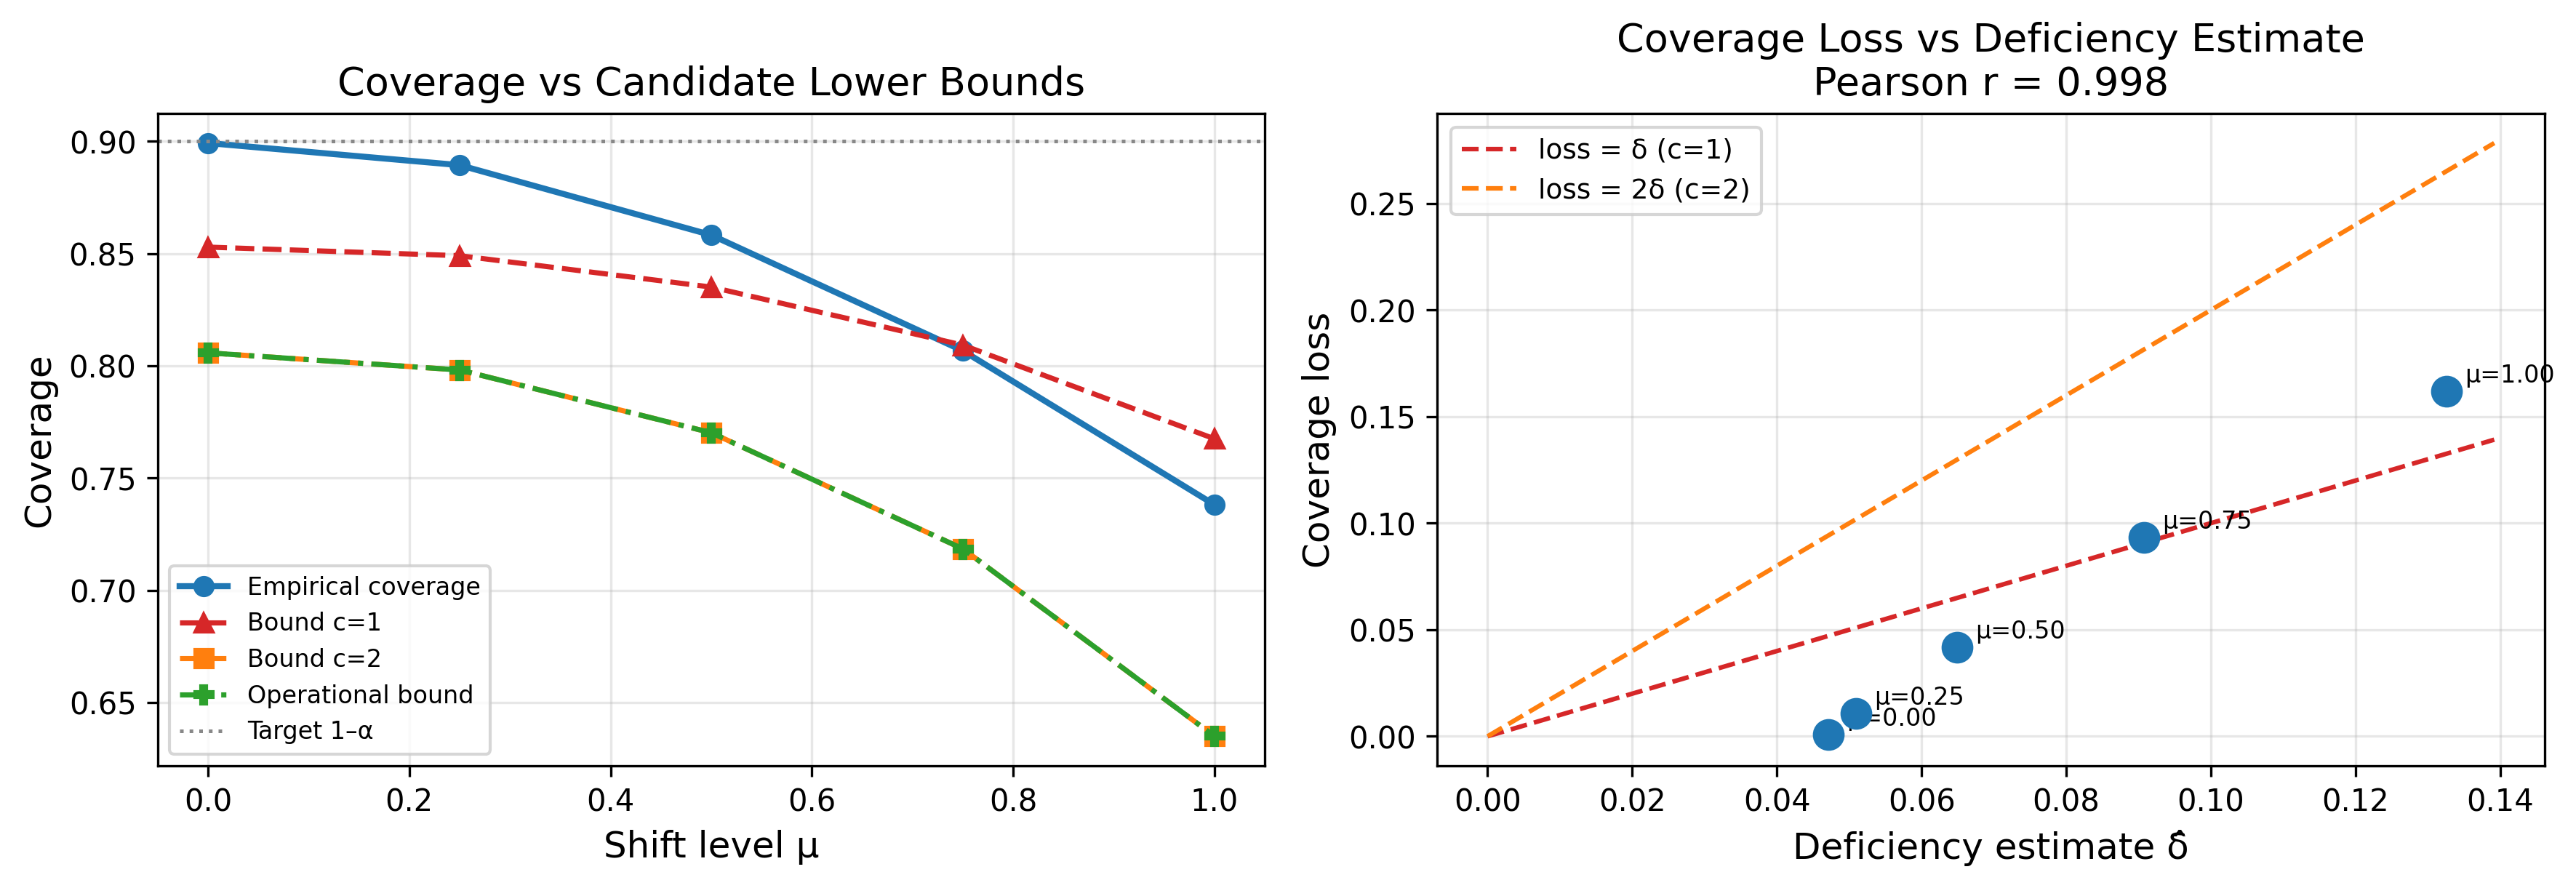
\includegraphics[width=0.92\linewidth]{figures/validate_theorem1.png}
\caption{Synthetic study: coverage, candidate bounds and $\hat\delta$ against $\mu$.}
\end{figure}

\begin{figure}[t]
\centering
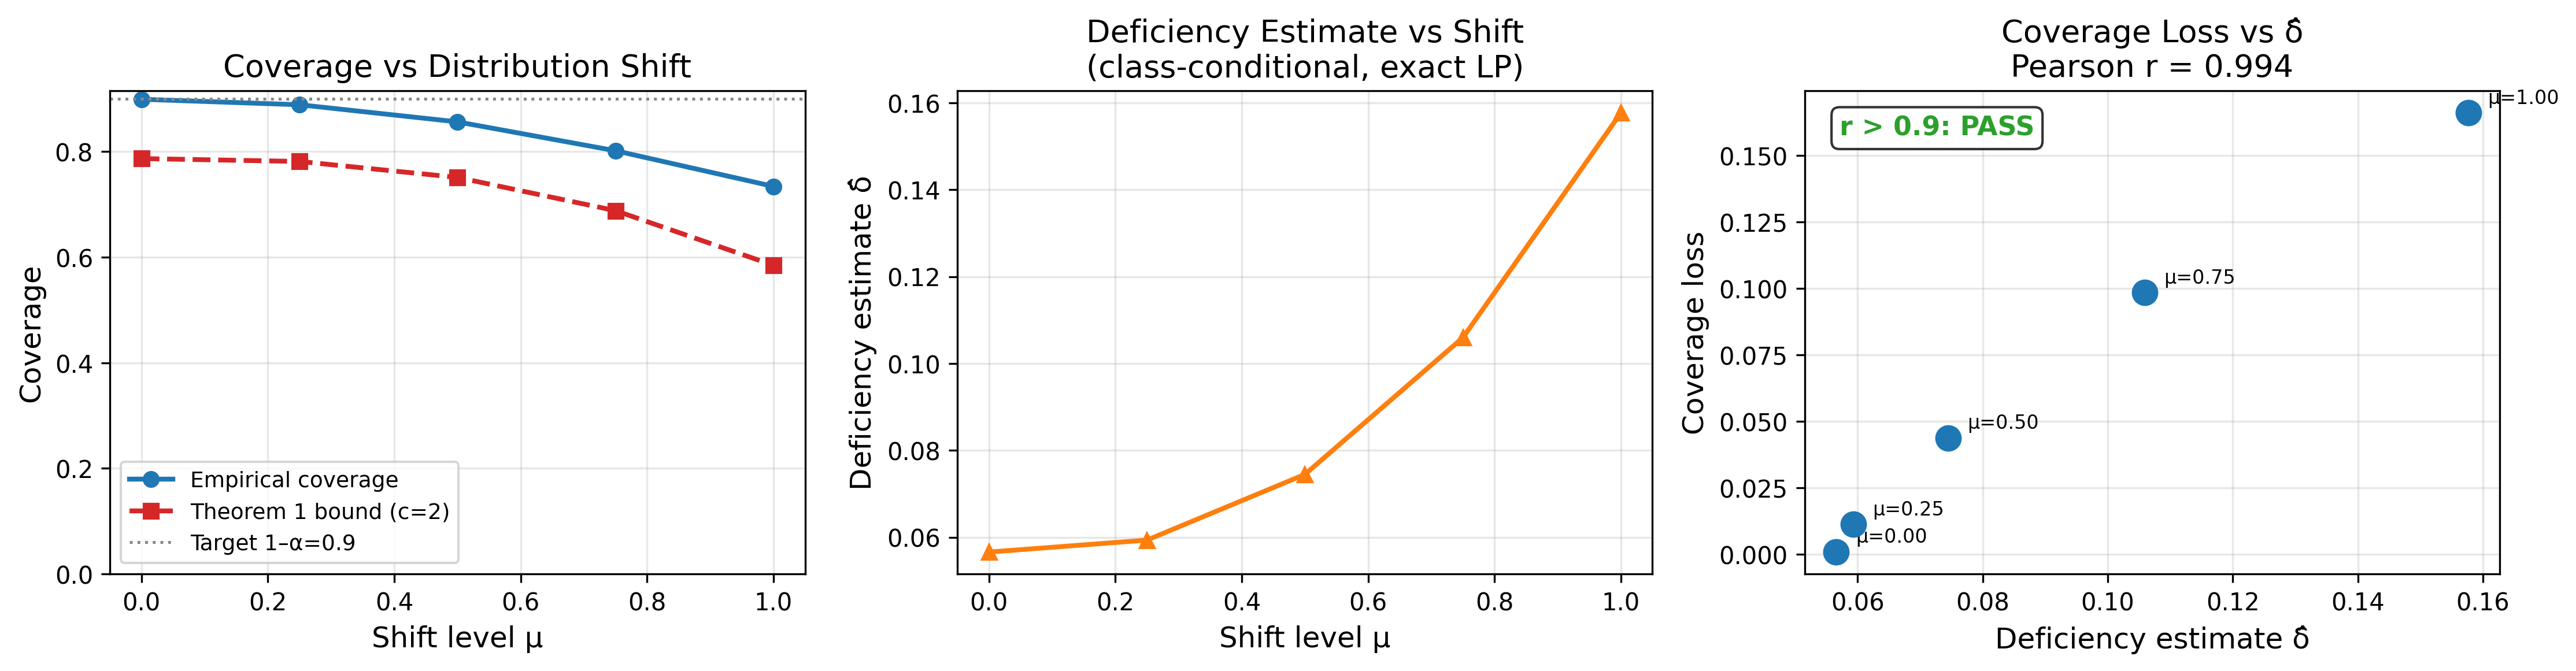
\includegraphics[width=0.92\linewidth]{figures/validate_drift_deficiency.png}
\caption{Coverage loss against $\hat\delta$ in the second synthetic experiment.}
\end{figure}

\subsection{\texorpdfstring{Is $\mathrm{TV}\le2\hat\delta$ true?}{Is TV <= 2 delta-hat true?}}
\label{sec:tvgap}

Two classes, same design, 30 trials, exact LP (\texttt{validate\_tv\_gap.py}).

\begin{table}[t]
\centering\small
\begin{tabular}{cccccc}
\toprule
$\mu$ & true TV & $\hat\delta$ (12 bins) & $\hat\delta$ (50 bins) & $\mathrm{TV}\le2\hat\delta$ & $c=2$ bound violated (12/50 bins) \\
\midrule
0.00 & 0.000 & 0.0060 & 0.0062 & 100\% & 30\% / 30\% \\
0.25 & 0.100 & 0.0069 & 0.0073 & 0\% & 53\% / 50\% \\
0.50 & 0.197 & 0.0086 & 0.0110 & 0\% & 93\% / 87\% \\
0.75 & 0.292 & 0.0114 & 0.0179 & 0\% & 100\% / 100\% \\
1.00 & 0.383 & 0.0170 & 0.0301 & 0\% & 100\% / 100\% \\
\bottomrule
\end{tabular}
\caption{Ground-truth check. Fraction of trials in which the theorem's hypothesis
holds, and in which the $c=2$ coverage bound is violated.}
\label{tab:tvgap}
\end{table}

The hypothesis fails in every trial for $\mu\ge0.25$, in line with
Proposition~\ref{prop:defbound}: the continuous class-conditional
experiment has deficiency zero here, and the nonzero values are
discretisation and sampling effects. (At $\mu=0$ the
``violations'' are ordinary sampling variation of empirical coverage around
$0.9$ against a bound only slightly below $0.9$.)

\subsection{Cross-domain tabular benchmark (UCI Covertype)}

The calibration domain is Wilderness Area 1; each of the four areas is
evaluated on 4000 held-out rows ($n_{\mathrm{cal}}=8000$, $n_{\mathrm{train}}=12000$).
Wilderness Area 1 is the in-distribution control. Means over the four rows:
coverage $0.8392$, coverage loss $0.0608$, ECE $0.0451$, $\hat\delta=0.1774$.

\begin{table}[t]
\centering\small
\begin{tabular}{lcccc}
\toprule
Domain & $n$ & Coverage & ECE & $\hat\delta$ \\
\midrule
wilderness\_1 & 4000 & 0.899 & 0.019 & 0.005 \\
wilderness\_2 & 4000 & 0.796 & 0.095 & 0.316 \\
wilderness\_3 & 4000 & 0.854 & 0.032 & 0.035 \\
wilderness\_4 & 4000 & 0.808 & 0.034 & 0.354 \\
\bottomrule
\end{tabular}
\caption{UCI Covertype (exact LP, 5 bins, seed 42).}
\label{tab:covertype}
\end{table}

The two domains with the largest $\hat\delta$ are the two with the largest
coverage loss. With four domains this is weak evidence: Pearson
$r=0.925$ ($p=0.075$), Spearman $\rho=0.80$ ($p=0.20$). The threshold
$\hat\delta>0.3$ separates the domains here but was chosen after seeing them.

\begin{figure}[t]
\centering
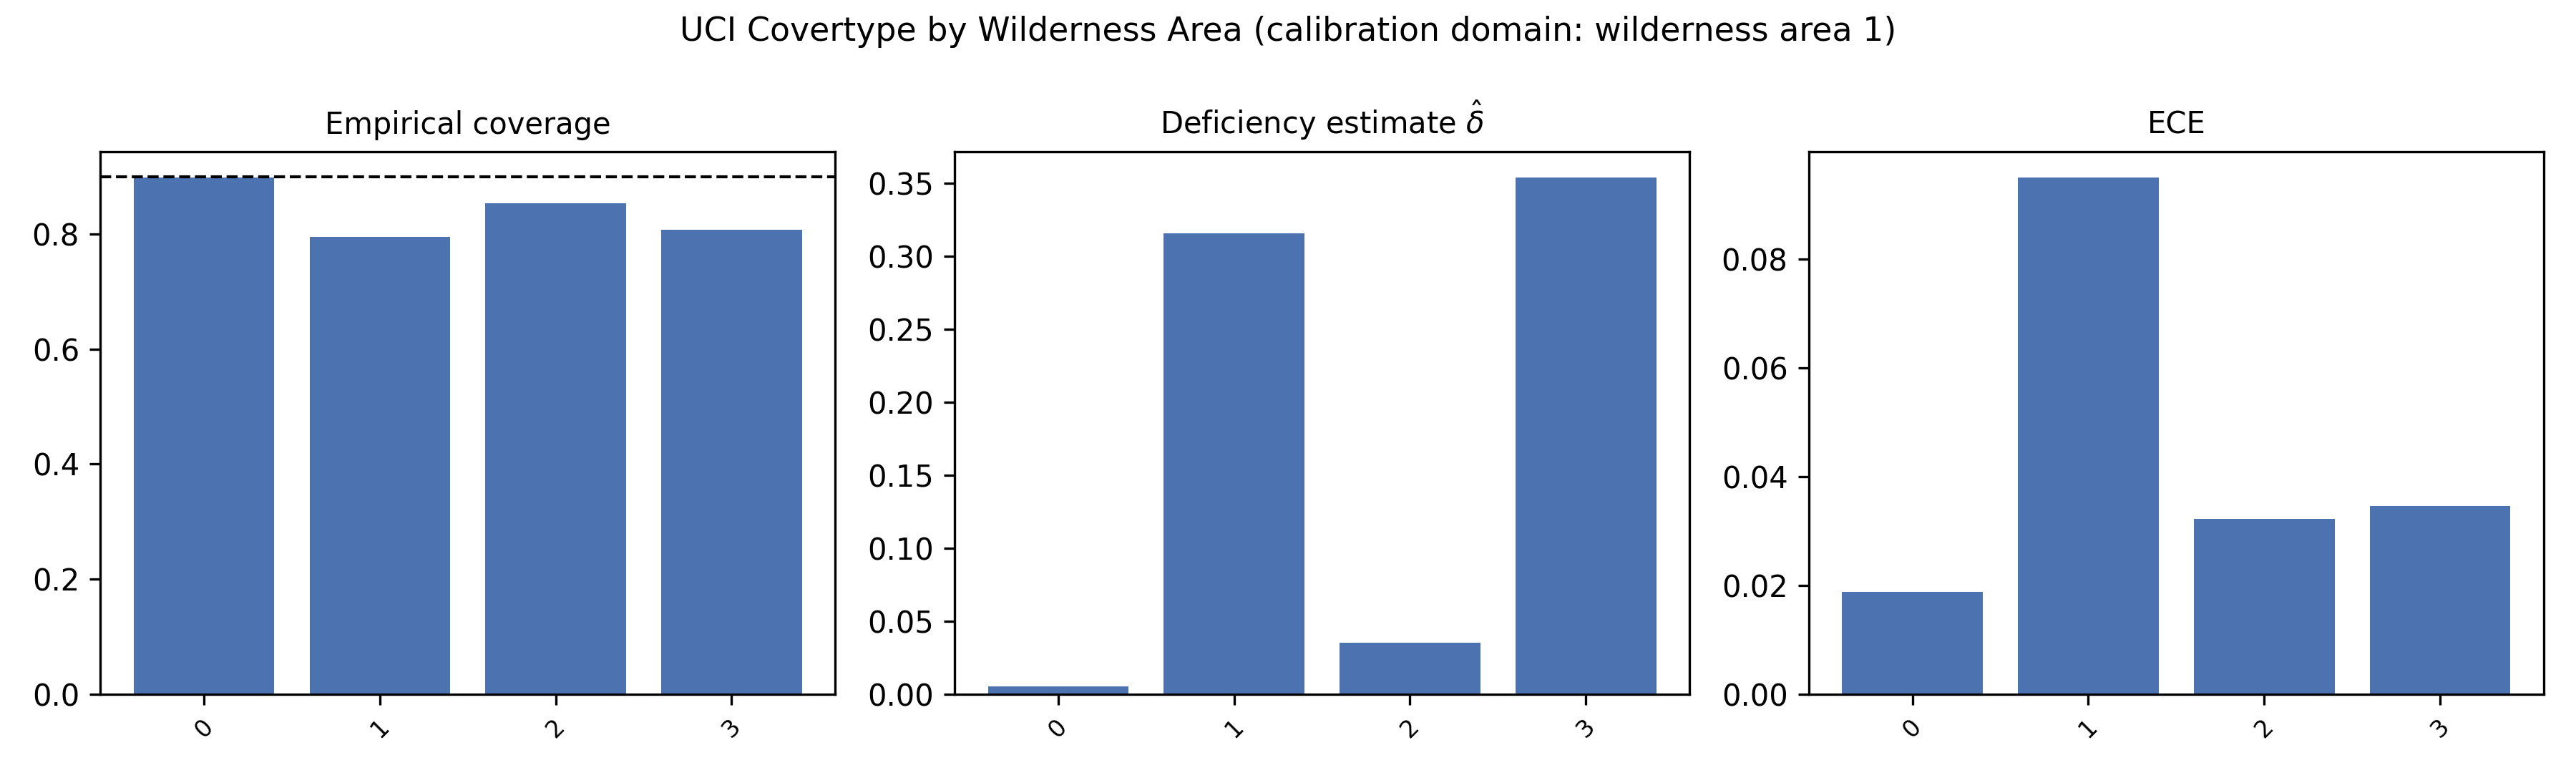
\includegraphics[width=0.95\linewidth]{figures/camelyon_fallback_domain_metrics.png}
\caption{Covertype: coverage, $\hat\delta$ and ECE by domain.}
\end{figure}

\subsection{Cross-domain text benchmark (20 Newsgroups)}

Topic-prefix groups are the domains; the calibration domain is \texttt{comp}
($n_{\mathrm{cal}}=1468$, $n_{\mathrm{train}}=9846$). Means over seven domains:
coverage $0.9511$, ECE $0.3307$, $\hat\delta=0.0943$.

\begin{table}[t]
\centering\small
\begin{tabular}{lcccc}
\toprule
Domain & $n$ & Coverage & ECE & $\hat\delta$ \\
\midrule
alt  & 319  & 0.953 & 0.201 & 0.084 \\
comp & 1955 & 0.872 & 0.269 & 0.010 \\
misc & 390  & 0.982 & 0.365 & 0.098 \\
rec  & 1590 & 0.990 & 0.420 & 0.138 \\
sci  & 1579 & 0.979 & 0.416 & 0.121 \\
soc  & 398  & 0.950 & 0.407 & 0.095 \\
talk & 1301 & 0.932 & 0.237 & 0.115 \\
\bottomrule
\end{tabular}
\caption{20 Newsgroups (exact LP, 5 bins, seed 42).}
\label{tab:news}
\end{table}

Only \texttt{comp} falls below the nominal $0.9$ and it has the \emph{smallest}
$\hat\delta$. The benchmark script defines coverage loss as
$\max\{0,\,0.9-\text{coverage}\}$, which is zero for the other six domains,
so the correlation across the seven domains ($r=-0.90$; $r=-0.88$ with the
unclipped difference $0.9-\text{coverage}$) records only that the one
under-covering domain has the smallest $\hat\delta$. On this benchmark
$\hat\delta$ does not track coverage loss. High ECE
($0.20$--$0.42$) coexists with near-nominal coverage, as expected since
conformal sets do not depend on probability calibration. We have not
established why \texttt{comp} under-covers; sampling variation and the way
the calibration and test \texttt{comp} splits were drawn are both candidates.
Whether $\hat\delta$ measures label-conditional shift here is also limited by
the domains being defined by label groups.

\begin{figure}[t]
\centering
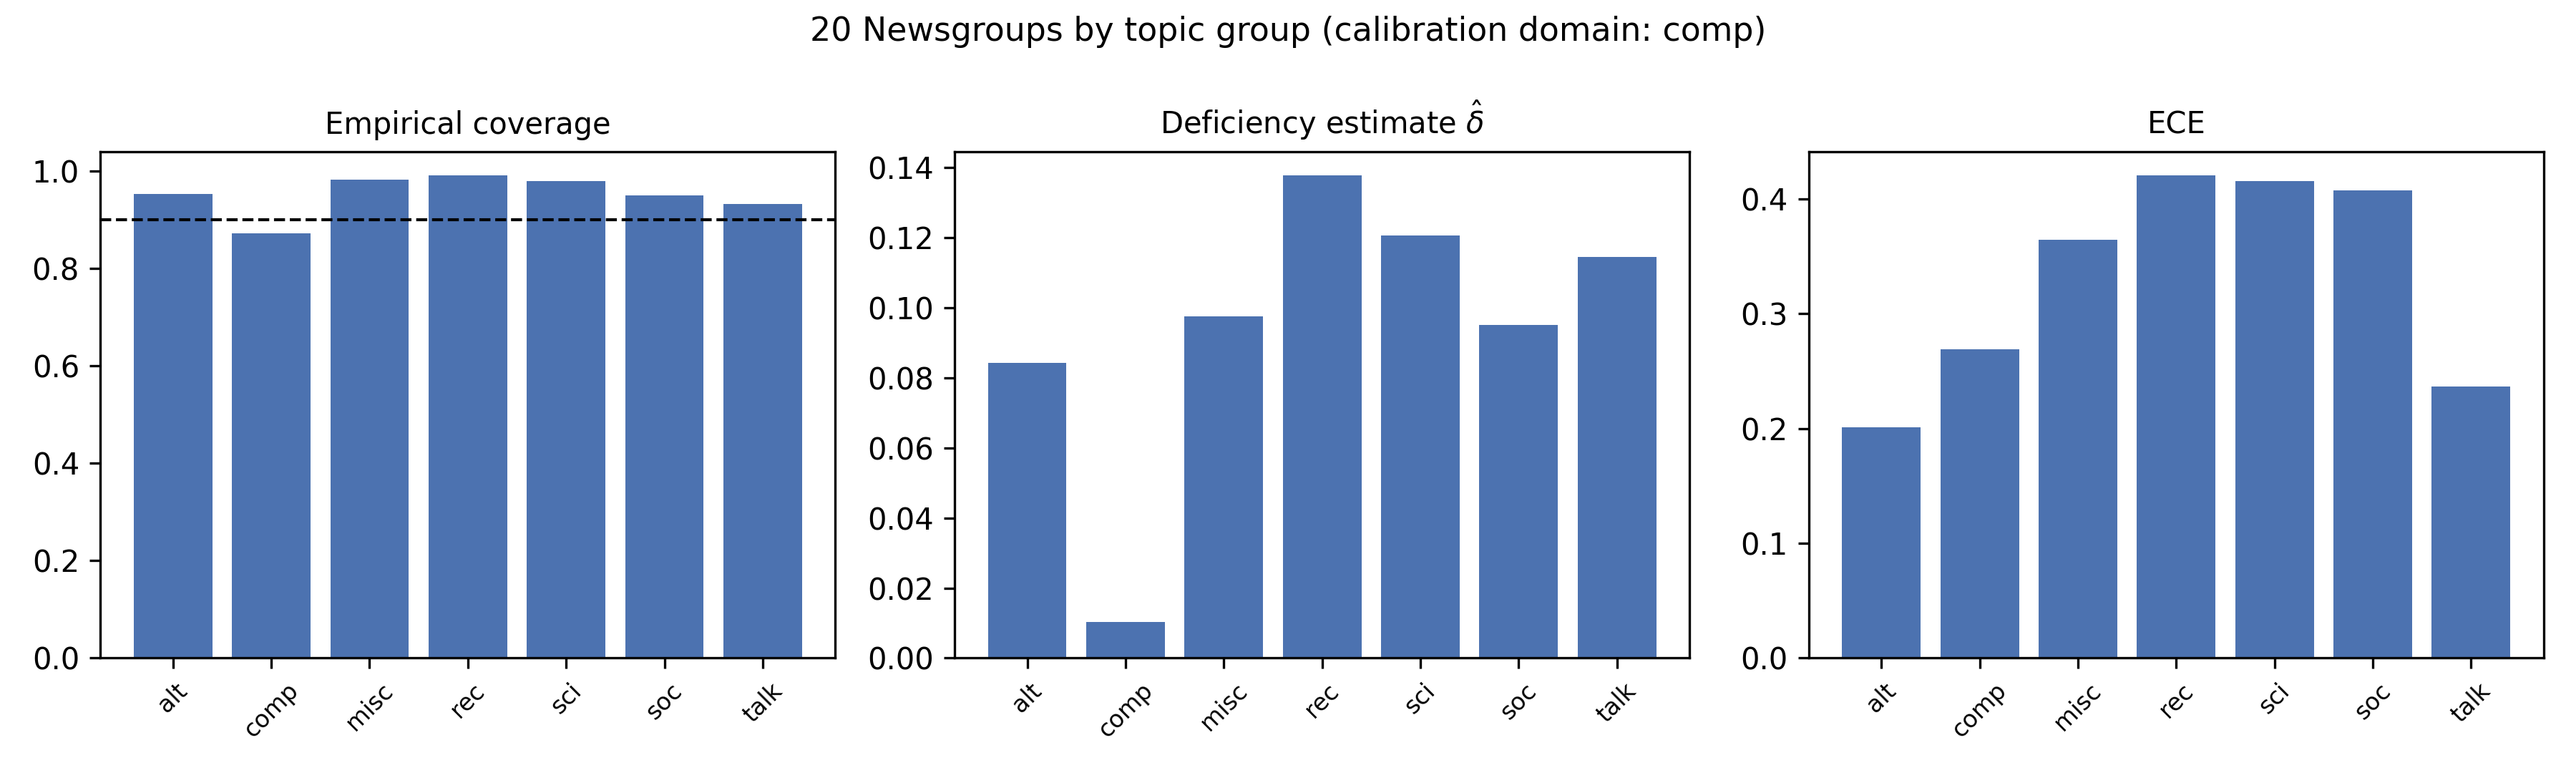
\includegraphics[width=0.95\linewidth]{figures/amazon_fallback_domain_metrics.png}
\caption{20 Newsgroups: coverage, $\hat\delta$ and ECE by domain.}
\end{figure}

\subsection{Substitute datasets}
Native WILDS Camelyon17 and Amazon were not available locally; the two
benchmarks above are substitutes and are not WILDS-distributed. Camelyon17 and
Amazon runs end as ``blocked'' in \texttt{experiments/results}.

\section{Related work}
Weighted conformal prediction \citep{tibshirani2019conformal} restores exact
coverage under covariate shift by reweighting the calibration scores with the
covariate likelihood ratio $d\Ptest/d\Pcal$; it needs that ratio and assumes
$P(Y\mid X)$ unchanged, whereas we assume nothing about the form of the shift
and ask only how much coverage can be lost. Adaptive conformal inference
\citep{gibbs2021adaptive} adjusts the miscoverage level online from observed
coverage errors and attains the target rate on average over time; it is a
feedback control scheme, not a bound for a fixed predictor. The analysis
beyond exchangeability of \citet{barber2023conformal} bounds the coverage gap
of weighted conformal sets by a weighted sum of TV distances between the joint
law of the $n+1$ points and its one-swap permutations; Theorem~\ref{thm:tv}
is the elementary two-law statement of that type, and our contribution is not
the bound but the test of whether a deficiency estimate can stand in for the
TV. Domain-adaptation theory \citep{bendavid2010theory} bounds target risk by
a source--target discrepancy over a hypothesis class; deficiency is instead a
discrepancy between experiments indexed by the label. We differ from all of
these in asking whether a Le Cam deficiency estimate can serve as a monitor,
and in documenting that it cannot serve as a certificate.

\section{Limitations and conclusion}
The only guarantee we prove is the TV bound, and TV between continuous
distributions cannot be certified from samples without further assumptions.
The deficiency estimate is not an upper bound on TV, requires test labels, is
blind to label-prior shift, depends on the discretisation, and behaved
opposite to coverage loss on one of two real benchmarks. It is best read as an
uncertified screening statistic. A principled certificate would need either a
TV estimator with a stated assumption on the discretisation or a recalibration
procedure that transports calibration data through the fitted kernel; neither
is attempted here.

\appendix
\section{Proof of Proposition~\ref{prop:tight}}
\label{app:tight}
Let $\Pcal(B)=\alpha$, $\Pcal^B=\Pcal(\cdot\mid B)$, $\Pcal^{B^c}=\Pcal(\cdot\mid B^c)$.
Since $\varepsilon\le1-\alpha$, $\Ptest=(\alpha+\varepsilon)\Pcal^B+(1-\alpha-\varepsilon)\Pcal^{B^c}$
is a probability measure with $\Ptest(B)=\alpha+\varepsilon$. Also
$\Ptest-\Pcal=\varepsilon(\Pcal^B-\Pcal^{B^c})$ and the two conditional laws have
disjoint supports, so $\TV{\Pcal}{\Ptest}=\varepsilon$. \qed

\section{Proof of Proposition~\ref{prop:defbound}}
\label{app:defbound}
(1) Take $K=I$. (2) If the supports $S_\theta$ of the $P_\theta$ are disjoint,
define $K(x,\cdot)=Q_\theta$ for $x\in S_\theta$ and arbitrary elsewhere. Then
$KP_\theta=Q_\theta$ for every $\theta$, so $\delta=0$. \qed

\bibliographystyle{unsrtnat}
\bibliography{refs}
\end{document}
